\documentclass[letterpaper, 12pt, parskip=full, headsepline]{scrartcl}
% Title and Subtitle added in .tex file
\title{Optimal Policies to Battle the Coronavirus ``Infodemic'' Among Social Media Users in Sub-Saharan Africa}
\subtitle{Preanalysis plan}
\author{Susan Athey, Molly Offer-Westort, Leah R. Rosenzweig}
\date{\today}

% USE: %\documentclass[letterpaper, 12pt, parskip=full,]{scrartcl}

\RequirePackage{etex}

% Graphics
\RequirePackage{graphicx}
\RequirePackage{epsfig}
\RequirePackage{psfrag}
\RequirePackage{wrapfig}
\RequirePackage[all]{xy}
\RequirePackage{listings}
\RequirePackage{verbatim} 
\RequirePackage{color} 
% Bold the 'Figure #' in the caption and separate it from the title/caption with a period
% Captions will be left justified
\RequirePackage[aboveskip=1pt,labelfont=bf,labelsep=period,justification=raggedright,singlelinecheck=off]{caption}


% Tables
\RequirePackage{float}
\RequirePackage{rotating}
\RequirePackage{array}
%\RequirePackage{minipage}
\RequirePackage{booktabs,threeparttable}

% Author
\RequirePackage[blocks]{authblk}
\renewcommand\Affilfont{\small}
\setlength{\affilsep}{0em}

\lstset{breaklines=true,basicstyle=\footnotesize\ttfamily}

% Document formatting
%\RequirePackage{fullpage}
\RequirePackage{setspace}
\RequirePackage{mathptmx}
\RequirePackage[hyphens]{url}
\RequirePackage{microtype} 
\RequirePackage[utf8x]{inputenc}
\RequirePackage{enumitem}
\setlist[itemize]{noitemsep, topsep=0pt}
\RequirePackage[colorinlistoftodos, textsize=footnotesize, color=blue!20!white]{todonotes} % adding to-do notes in working file
%\addtokomafont{disposition}{\normalfont\bfseries} % article fonts
%\setkomafont{descriptionlabel}{\normalfont\bfseries} % article fonts

% Bibliography and citation formatting
\RequirePackage[colorlinks=true, citecolor=blue]{hyperref}

\RequirePackage{nameref}
\RequirePackage[round]{natbib} 
\bibliographystyle{chicago}

% Title and Subtitle added in .tex file
%\author{Molly Offer-Westort}
%\date{\today}

\makeatletter %Set \Title reference
\let\Title\@title
\makeatother

\makeatletter %Set \Subtitle reference
\let\Subtitle\@subtitle
\makeatother

\makeatletter %Set \Author reference
\let\Author\@author
\makeatother

% Header and Footer
\RequirePackage{scrlayer-scrpage}
%\ihead{\textbf{\Title} }
%\ohead{\Author}

\RequirePackage{lastpage}
%\cfoot[]{}
%\ofoot[]{\thepage\ of \pageref{LastPage}}
\pagestyle{scrheadings}
%\setkomafont{pageheadfoot}{\small}
\RequirePackage{footnote}
\deffootnote[1.5em]{.5em}{1em}{\textsuperscript{\thefootnotemark}}


% Equation formatting
\RequirePackage{amsmath,amssymb,amsfonts} 
\RequirePackage{amsthm}
\RequirePackage{bbm}
\RequirePackage{array}
\newcommand\numberthis{\addtocounter{equation}{1}\tag{\theequation}}

\newtheorem{theorem}{Theorem}[section]
\newtheorem{lemma}{Lemma}[section]
\newtheorem{prop}{Proposition}[section]
\newtheorem{corollary}{Corollary}[section]
\newtheorem{hypothesis}{Hypothesis}


% Shortcuts
\newcommand{\nn}{\nonumber}

% Define new characters
\def\Var{{\textrm{Var}}\,}
\def\V{{\textrm V}\,}
\def\E{{\textrm E}\,}
\def\arg{{\textrm {arg} }\,}
\def\Cov{{\textrm{Cov} }\,}
\def\Cor{{\textrm{Cor} }\,}
\def\N{{\textrm N}\,}
\def\Supp{{\textrm {Supp} }\,}
\DeclareMathOperator*{\argmin}{arg\,min}
\DeclareMathOperator*{\argmax}{arg\,max}

%--------------------------------------------------------------------------
% Math boldface shortcuts, etc. ----------------------------------
%--------------------------------------------------------------------------
\newcommand{\A}{\mathbf{A}}\newcommand{\B}{\mathbf{B}}\newcommand{\C}{\mathbf{C}}
\newcommand{\D}{\mathbf{D}}\newcommand{\F}{\mathbf{F}}\newcommand{\G}{\mathbf{G}}
\newcommand{\HB}{\mathbf{H}}\newcommand{\I}{\mathbf{I}}\newcommand{\J}{\mathbf{J}}
\newcommand{\K}{\mathbf{K}}\newcommand{\Lb}{\mathbf{L}}\newcommand{\M}{\mathbf{M}}
\newcommand{\NB}{\mathbf{N}}\newcommand{\OB}{\mathbf{O}}\newcommand{\PB}{\mathbf{P}}
\newcommand{\Q}{\mathbf{Q}}\newcommand{\R}{\mathbf{R}}\newcommand{\SB}{\mathbf{S}}
\newcommand{\T}{\mathbf{T}}\newcommand{\U}{\mathbf{U}}%\newcommand{\V}{\mathbf{V}}
\newcommand{\W}{\mathbf{W}}\newcommand{\X}{\mathbf{X}}\newcommand{\Y}{\mathbf{Y}}
\newcommand{\Z}{\mathbf{Z}}

\newcommand{\aB}{\mathbf{a}}\newcommand{\bB}{\mathbf{b}}\newcommand{\cB}{\mathbf{c}}
\newcommand{\dB}{\mathbf{d}}\newcommand{\e}{\mathbf{e}}\newcommand{\f}{\mathbf{f}}
\newcommand{\g}{\mathbf{g}}\newcommand{\h}{\mathbf{h}}\newcommand{\iB}{\mathbf{i}}
\newcommand{\jB}{\mathbf{j}}\newcommand{\kB}{\mathbf{k}}\newcommand{\lB}{\mathbf{l}}
\newcommand{\m}{\mathbf{m}}\newcommand{\n}{\mathbf{n}}\newcommand{\oB}{\mathbf{o}}
\newcommand{\p}{\mathbf{p}}\newcommand{\q}{\mathbf{q}}\newcommand{\rB}{\mathbf{r}}
\newcommand{\s}{\mathbf{s}}\newcommand{\tB}{\mathbf{t}}\newcommand{\uB}{\mathbf{u}}
\newcommand{\vB}{\mathbf{v}}\newcommand{\w}{\mathbf{w}}\newcommand{\x}{\mathbf{x}}
\newcommand{\y}{\mathbf{y}}\newcommand{\z}{\mathbf{z}}

\def\AA{{\mathbb A}}\def\BB{{\mathbb B}}\def\CC{{\mathbb C}}
\def\DD{{\mathbb D}}\def\EE{{\mathbb E}}\def\FF{{\mathbb F}}
\def\GG{{\mathbb G}}\def\HH{{\mathbb H}}\def\II{{\mathbb I}}
\def\JJ{{\mathbb J}}\def\KK{{\mathbb K}}\def\LL{{\mathbb L}}
\def\MM{{\mathbb M}}\def\NN{{\mathbb N}}\def\OO{{\mathbb O}}
\def\PP{{\mathbb P}}\def\QQ{{\mathbb Q}}\def\RR{{\mathbb R}}
\def\SS{{\mathbb S}}\def\TT{{\mathbb T}}\def\UU{{\mathbb U}}
\def\VV{{\mathbb V}}\def\WW{{\mathbb W}}\def\XX{{\mathbb X}}
\def\YY{{\mathbb Y}}\def\ZZ{{\mathbb Z}}

\RequirePackage{euscript}
\let\muchmore= \gg
\let\muchless= \ll
\let\typewriter=\tt  % for turning on the typewriter font
\def\aa{{\EuScript A}}\def\bb{{\EuScript B}}\def\cc{{\EuScript C}}\def\dd{{\EuScript D}}
\def\ee{{\EuScript E}}\def\ff{{\EuScript F}}\def\gg{{\EuScript G}}\def\hh{{\EuScript H}}
\def\ii{{\EuScript I}}\def\jj{{\EuScript J}}\def\kk{{\EuScript K}}\def\ll{{\EuScript L}}
\def\mm{{\EuScript M}}\def\nn{{\EuScript N}}\def\oo{{\EuScript O}}\def\pp{{\EuScript P}}
\def\qq{{\EuScript Q}}\def\rr{{\EuScript R}}\def\ss{{\EuScript S}}\def\tt{{\EuScript T}}
\def\uu{{\EuScript U}}\def\vv{{\EuScript V}}\def\ww{{\EuScript W}}\def\xx{{\EuScript X}}
\def\yy{{\EuScript Y}}\def\zz{{\EuScript Z}}

\newcommand{\Beta}{\boldsymbol{\beta}}
\newcommand{\btheta}{\boldsymbol{\theta}}
\newcommand{\bgamma}{\boldsymbol{\gamma}}
\newcommand{\bpi}{\boldsymbol{\pi}}
\newcommand{\arrowp}{\stackrel{p}{\rightarrow}}
\newcommand{\0}{\mathbf{0}}
\newcommand{\bP}{\mathbf{P}}

\newcommand\independent{\protect\mathpalette{\protect\independenT}{\perp}}
\def\independenT#1#2{\mathrel{\rlap{$#1#2$}\mkern2mu{#1#2}}}


\newcommand{\indep}{\perp\!\!\!\!\perp}

\thispagestyle{plain}



\begin{document}%
\normalsize%
\maketitle%
\tableofcontents%
\clearpage%


\begin{abstract}
Alongside the outbreak of Coronavirus, much of the world’s population is also experiencing an “infodemic” -- the spread of myths and hoax cures related to the virus. Covid-19 misinformation is spreading through online media outlets and social media platforms. While many false cures are largely harmless (e.g., drinking lemon water), others have devastating consequences, such as taking chloroquine. As a result, governments struggling to prepare healthcare systems and encourage citizens to comply with best practices also need to tackle misinformation. Building upon the experimental literature on combating fake news, we evaluate the effect of interventions designed to decrease sharing of false COVID-19 cures. Using Facebook advertisements to recruit social media users in Kenya and Nigeria, we deliver our interventions using a Facebook Messenger chatbot, allowing us to observe treatment effects in a realistic setting. Our aim is to find the context-aware intervention policy that will assign individuals the intervention that is most effective for them, based on their covariate profile. Using a contextual adaptive experimental design to sequentially assign treatment probabilities, we are able to learn the optimal contextual policy, and minimize assignment to ineffective or counter-productive interventions within the experiment. Analyzing heterogeneity in treatment effects allows us to learn whether different interventions are more effective for different people, improving our understanding of how to tackle harmful misinformation during an ongoing health crisis. Finally, we bring comparative data to a global problem for which the existing research has largely been limited to the Global North. This pre-analysis plan describes the research design and outlines the key hypotheses that we will evaluate.
\end{abstract}





\section{Motivation and Research Questions}

% motivation
Alongside the outbreak of Coronavirus, much of the world's population is also experiencing an ``infodemic'' -- the spread of myths and hoax cures related to the virus. Covid-19 misinformation is spreading through online media outlets and social media platforms. These falsities range from incorrect information about government action to hoax cures, some of which are largely harmless, such as drinking lemon water, while others can have devastating consequences if adopted, such as taking chloroquine or drinking bleach. As a result, governments struggling to prepare healthcare systems and encourage citizens to comply with best practices are also struggling to tackle a pandemic of misinformation.

% what we do 
This project evaluates the effect of interventions designed to decrease sharing of false COVID-19 cures. Using Facebook advertisements to recruit social media users in Kenya and Nigeria, we deliver our interventions using a Facebook Messenger chatbot, allowing us to observe treatment effects in a realistic setting. We test interventions targeted at both the respondent level, such as general warnings and headline-level treatments, such as flags and ``false'' tags (treatments are described in table \ref{tab:treatments}). 

Using a contextual adaptive experimental design, we sequentially assign treatment probabilities in order to learn the optimal contextual policy, and minimize assignment to ineffective or counter-productive interventions within the experiment. Our aim is to find the context-aware intervention policy that will assign individuals the intervention that is most effective for them, based on their covariate profile. Analyzing heterogeneity in treatment effects allows us to learn whether different interventions are more effective for different people, improving our understanding of how to tackle harmful misinformation during an ongoing health crisis. 

%% LR: we will also interact/factorialize the treatments and evaluate the best "policy" -which could be a combination of both respondent and headline-level interventions, right? If so, that's also a selling point!


% how we build on existing lit
This work builds on the experimental literature on combating fake news in several important ways. First, we examine several prominent interventions that have proven successful in other studies and in other settings and use an adaptive design to observe the best intervention policy. Second, we bring comparative data to a global problem for which the existing research has largely been limited to the Global North. Finally, This pre-analysis plan describes the research design and outlines the key hypotheses that we will evaluate.




\section{Case Selection}
% Why kenya + Nigeria?

We examine these questions using a study focused on online social media users in two of the major hubs of online communication in sub-Saharan Africa, Kenya and Nigeria. Collectively, these countries host 38 million Facebook users who are 18 years and older (as reported on Facebook's advertising platform). Misinformation and fake news are major problems in these countries. AfricaCheck.org, a third party verification site, has offices in both countries and has recently created pages devoted to COVID-19-related misinformation circulating online. 

%% LR: I'm looking for citations to demonstrate these are hubs of misinfo - another way to go is that they are major english media sources and other countries in the region often also read news from ky/ng...

\begin{figure}[htb]
\centering
\caption{Map illustrating the volume of fact-checks in \url{poynter.org}'s global coronavirus facts database.}
\label{fig:poynter}
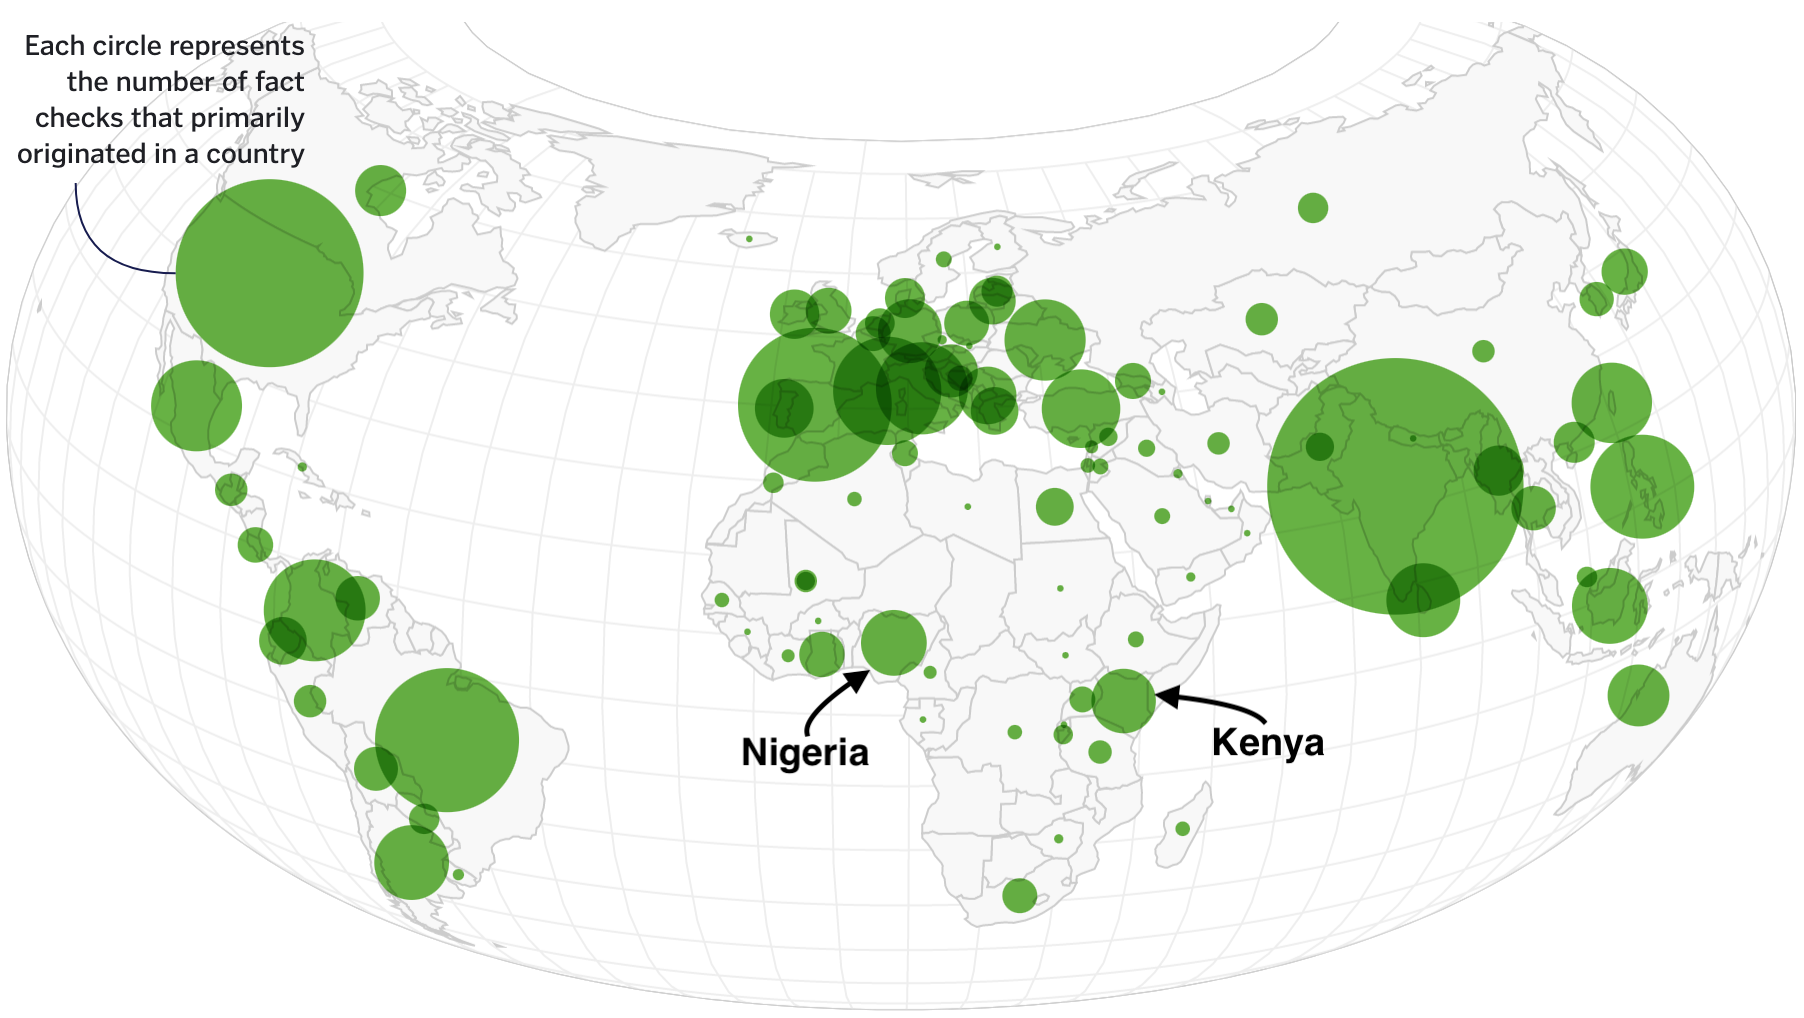
\includegraphics[width=.95\textwidth]{poynter2.png}
\end{figure}


\section{Research Design and Hypotheses}



\subsection{Sample recruitment}
We will recruit respondents in Kenya and Nigeria using Facebook advertisements targeted to users 18 years and older living in these countries.\footnote{Based on previous work it is clear that Facebook imputes location information for some of its users, which can be inaccurate. We will also ask a location screening question to ensure our respondents live in our countries of interest.} To achieve balance on gender within our sample we create separate ads targeting men and women in both countries. 

%% LR: do we want to achieve balance on any other demographics? Maybe some of the key variables we care about for the contextual bandit..? In my experience if we just create male/female country-level ads we'll also get mostly young, educated, urban respondents. But that's also largely who the FB population is (at least in kenya). But we could easily create more ads to get fill other quotas, but not sure if/how that will affect the randomization in the chatbot

After clicking on our advertisement that will offer users with the opportunity to ``Take a short COVID-19 survey for airtime,'' users will be directed to our Facebook page [link?] to interact with a Facebook Messenger chatbot. In contrast to sending users to a Qualtrics survey, the chatbot has the benefit of keeping users on the Facbeook platform, with which they are likely more familiar, and maintaining a realistic setting in which users might encounter online misinformation.\footnote{INCLUDE IN APPENDIX IMAGE OF AD + CHATBOT.} Respondents who complete the \textbf{20} minute survey in the chatbot will receive compensation in the form of mobile phone airtime sent to their phone. 

\subsection{Experimental setup}
The survey conducted through the chatbot involves an adaptive design to test the best performing intervention to tackle Covid misinformation. 

\subsubsection{Treatment}
Drawing on the literature on experimental interventions to combat misinformation, we include several interventions designed to reduce the spread of misinformation online, which are targeted both at the headline level and respondent level. 

%% LR: I can clean this up later - I wonder if we also want to have a column for previous studies that have used these treatments + their findings?
\begin{table}[htb!]
\begin{tabular}{l|l|l}
\multicolumn{1}{c|}{\textbf{\begin{tabular}[c]{@{}c@{}}Shorthand\\ Name\end{tabular}}} & \multicolumn{1}{c|}{\textbf{\begin{tabular}[c]{@{}c@{}}Treatment\\ Level\end{tabular}}} & \textbf{Treatment}                                                                                                                                                                                                                                                                                                                                                                                              \\ \hline
Facebook tips                                                                                                           & Respondent                                                                                                   &  Facebook's ``Tips to Spot False News'' 
\\
AfricaCheck tips                                                                                                         & Respondent                                                                                                   &  \url{Africacheck.org}'s guide: \\ & & ``How to vet information during a pandemic''                                                                                                                                                                                                                                                                                                                             \\
Video training                                                                                                     & Respondent                                                                                                   &  \href{https://www.bbc.com/news/av/embed/p088bh96/52118949}{BBC Video training}                                                                                                                                                                                                                                                                                                                                                                                  \\
Emotion suppression                                                                                                       & Respondent                                                                                                   & \begin{tabular}[t]{@{}l@{}}Prompt: ``As you view and read the headlines, if you have any \\feelings, please try your best not to let those feelings show.  \\Read all of the headlines carefully, but try to behave so that \\someone watching you would not know that you are feeling\\ anything at all.” \citep{gross1998emerging}\end{tabular}
\\
Accuracy nudge                                                                                 & Respondent                                                                                                   & Placebo headline: ``Do you think this headline accurately\\& & describes an event that actually  happened?'' \\& &  \citep{pennycook2020fighting}.
\\
Context                                                                                                        & Headline                                                                                                     & \begin{tabular}[t]{@{}l@{}}Facebook context button; if you click the info button on an\\ article, a pop-up tells you a few facts about the source: \\ how long the Facebook page has been registered,\\ and has a flag if article is more than 90 days old\end{tabular}
\\
Flag                                                                                                           & Headline                                                                                                     &  "Disputed" flag on the headline                                                                                                                                                                                                                                                                                                                                                     \\
Related articles                                                                                                       & Headline                                                                                                     & Facebook-style related stories: next to story link,\\ & & show two other stories which may confirm or correct the story                                                                                                                                                                                                                                                                                               \\
Factcheck                                                                                                      & Headline                                                                                                     & Fact checking score by third party\\ & & (e.g., Facebook, AFP, AfricaCheck, etc)
 \\
Control                                                                                                        & N/A                                                                                                          & Control condition                                                                                                                                                                                                                                                                                                                                                                                              
\end{tabular}
\caption{Description of interventions included in the experiment}
\label{tab:treatments}
\end{table}

% contextual bandit

% optimizing strategy/algorithm

\subsubsection{Outcomes}
We have two main outcomes of interest:

\begin{enumerate}
\item Willingness to read the article, as measured by the question: ``If it were possible, would you click this headline to read the full story?''
\item Interest in sharing the article, as measured by two questions. The first asks whether the respondent would like to post the article to their Facebook timeline and the second asks whether the respondent would like to send the article to a friend on Facebook. 
\end{enumerate}

In order to obtain a behavioral measure of sharing, we collect the articles the respondent indicated they would like to share throughout the survey and a the end of the survey provide links to the \textit{true} information. At this point we debrief the respondent, informing them that some (if any) of the headlines they wanted to share are \textit{false} and for that reason they are unable to share them. Instead, we provide links to tips for spotting misinformation online and links to the true pieces of information that they saw. By embedding variables in these urls we will be able to track if and how respondents shared these articles.


%% rather than it's own section we could also integrate hypotheses into the next section (analytic strategy)--e.g. say how we will analyze results and what we expect
\subsection{Hypotheses}
\subsubsection{Optimal interventions:}
\textbf{H1:} ...

\subsubsection{Heterogeneity:}
Analyzing heterogeneity in treatment effects allows us to learn whether different interventions are more effective for different people, improving our understanding of how to tackle harmful misinformation during an ongoing health crisis.
 
\textbf{H4:}...

\section{Analytic Strategy}
\subsection{Estimating Optimal}




%% below is leftover from the original adaptive preanalysis plan
\section{Policy learning and evaluation}

Following experimental data collection, personalized policies are estimated and evaluated modifying the method explained in \cite{athey2017efficient} and also in \cite{zhou2018offline}; in those approaches, data is collected non-adaptively and is assumed to be iid. In the adaptive setting, we can not make this assumption about the data. Instead, the sample is split into an initial training period on which we learn the optimal policy: given a class of functions $\Pi$, we fit an optimal policy that satisfies
\begin{align}
  \hat{\pi}_{EST} = \arg\max_{\pi \in \Pi} \frac{1}{n}\sum_{i} \langle \pi(X_{i}), \hat{\Gamma}_{i,\cdot} \rangle
\end{align}
where $\{\hat{\Gamma}_{i,k}\}_{k=1}^{|\mathcal{W}|}$ are doubly robust scores. 
%{\color{red}In this experiment, we will restrict our policy class $\Pi$ to be the set multinomial logistic cost-sensitive classifiers with L1-penalty.}

We then estimate the value of the policy on the remaining observations. This approach is described in further detail below. 

{\color{red} [This section needs to be clarified once we decide on an approach to policy learning.] }


\begin{enumerate}
%
  \item Divide the data in half, and then within each half, divide the data again into $K$ folds, denoted by $S_{[1]k}$ and $S_{[2]k}$ for $k = 1, \dots, K$. (We will assume without loss of generality that $n$ is even)
  %
  \item Within each fold $k$, estimate $\hat{\mu}_{w}(X_{i})$ from a model fit on the K-1 remaining folds. This model could be produced, e.g., using generalized random forests with sample splitting \citep{athey2016generalized}; {\color{red}[[Confirm how we're fitting at this point]]} 
  
  Also within each fold $k$, calculate balancing weights $\gamma$ from the procedure described in \ref{appendix:sample_balancing}. 
  
  \item Construct doubly-robust scores $\hat{\Gamma}_{i,w}$ within each fold from the $\hat{\mu}_{w}(X_{i})$ and $\gamma$ from the previous step, following the procedure described in \ref{appendix:doubly-robust}.  
  
  \item Concatenate doubly-robust scores within each half of the data to generate the $\frac n 2 \times |\mathcal{W}|$ matrices $\hat{\Gamma}_{[1]}$ and $\hat{\Gamma}_{[2]}$. 
  
  \item Estimate the optimal personalized policy within each half of the data for the given policy class, e.g., for the first half:
  \begin{align}
      \hat{\pi}_{[1]} := \arg\max_{\pi \in \Pi} \frac{1}{|S_{[1]}|} \sum_{i \in S_{[1]}} \langle \pi(X_{i}), \hat{\Gamma}_{[1]i,\cdot} \rangle
  \end{align}

  \item For each observation $i$, compute the predicted optimal assignment
      \begin{align}
       \hat{\pi}_{(-i)}(X_{i})
      \end{align}
  \noindent where the subscript indicates that we used the policy from the half of the data that did not contain $i$.
 
 \item For each half of the data, estimate {\color{red}value} $\widehat{Q}_1$ and $\widehat{Q}_2$, where, e.g., 
  \begin{align}
     \widehat{Q}_{1} := \frac{1}{|S_{[1]}|} \sum_{i \in S_{[1]}} \langle \hat{\pi}_{[2]}(X_{i}), \hat{\Gamma}_{[1]i,\cdot} \rangle
  \end{align}

\item Finally, we estimate the average value for the optimal personalized policy:

  {\color{red}
  \begin{align}
     \widehat{Q}(\widehat{\pi}) := \frac{1}{2} \left(   \widehat{Q}_{1} +   \widehat{Q}_{2}\right)
  \end{align}}

\end{enumerate}



\section{Matrix method, outcome model, and balancing weights}
\subsection{Matrix method} 
To estimate the value of a given policy, we may use an outcome model, weights, or both. Here, the estimated counterfactual rewards, $\{\hat{\Gamma}_{i,k}\}_{k=1}^{|\mathcal{W}|}$, may be estimated via,
\begin{itemize}
\item \textbf{Inverse probability weighted estimation}, using a version of Horvitz-Thompson estimator \citep{horvitz1952}
\begin{align}
\hat{\Gamma}_w^{HT} & =  \frac{1}{n} \sum_{i = 1}^n 1 \{ W_i = w\} \gamma_i Y_i. 
\end{align}
\item \textbf{Adaptively weighted doubly-robust estimation}. 
\label{appendix:doubly-robust}
\textcolor{red}{[To be further filled in, with reference to LFO paper.]}\\
We estimate an $n \times |\mathcal{W}|$ matrix of \textit{doubly-robust scores} $\hat{\Gamma}_{i,w}$. For each treatment $w$ and observation $i$, we compute    
      \begin{align}
        \hat{\Gamma}_{i,w} = \hat{\mu}_{w}(X_{i}) + 1 \{W_i = w \} \gamma_{i}(Y_{i} - \hat{\mu}_w(X_i))
    \end{align}
  The term involving the balancing weights, $\gamma_i$, is a correction that mitigates selection bias arising from not collecting the data by assigning treatments uniformly at random; approaches are discussed in Appendix~\ref{appendix:sample_balancing}. Each element of this matrix is a (corrected) estimate of the average reward that the observation $i$ would have received had they been given treatment $w$.
\end{itemize}



\subsection{Outcome model} The {outcome model} refers to the underlying statistical model used to predict the conditional mean and variance of rewards, $\hat{\mu}_w(X_{i}), \ \hat{\sigma}_w^2(X_{i})$ for all arms $w$, used in doubly-robust estimation. In simulations, we align the outcome model of the estimated policy with the agent assigned above. 

\begin{itemize}
\item \textbf{Ridge.} We use a linear model with treatment indicators, covariates, and treatment and covariates interacted:
\begin{align}
\hat{\mu}_w(X_{i}) = \hat{\beta}_{0} +
			\sum_{w} 1\{W_i = w\}\hat\beta_w  +
			\sum_{\ell}  X_{[\ell]i}\hat{\beta}_{\ell} +
         \sum_{w,\ell} 1\{ W_{i} = w\} X_{[\ell]i} \hat{\beta}_{w, \ell}.
         \label{eq:linear_model_full}
\end{align} 
The model is estimated using $L_{2}$ %or $L_{2}$ 
penalties for regularization, exclusive of the main treatment effects $\beta_{W,\cdot}$.

\item \textbf{Generalized random forest}.  Alternatively, we may train a random forest  %\footnote{Using the function \texttt{regression\_forest} from R package \texttt{grf}} 
on the entire history of subjects assigned to each arm $w$. Point predictions and their conditional variances are computed as described in \citet[section 4]{athey2016generalized}. 
\end{itemize}



\subsection{Balancing weights} To account for unequal treatment assignment probabilities, we use balancing weights, $\gamma_i$. 
\begin{itemize}\setlength\itemsep{0em}
\item \textbf{Batch-wise inverse probability weights} are detailed in Appendix~\ref{appendix:probability}. 
\item \textbf{Stabilized inverse probability weights} are detailed in Appendix~\ref{appendix:stabilized}.
\item \textbf{Approximate residual balancing weights} are detailed in Appendix~\ref{appendix:sample_balancing}.
\end{itemize}



%\subsection{Variance estimation}
%\textcolor{red}{[TBD]}



\subsection{Sample balancing}
\label{appendix:sample_balancing}

\subsubsection{Batch-wise inverse probability weighting} \label{appendix:probability}
Given a specific policy $\pi$, we can consider the probability of being assigned a treatment arm $w$ given a contextual variable $X_{i}$.
\begin{align}
e^{\pi}_{w}(X_i) := P(\pi(X_i) = w )
\label{eq:weighted_optimization}
\end{align}

In a bandit problem, this probability varies with the batch under which observation $i$ was collected, as the agent updates the probabilistic policy assigned using the past history. However, within each batch the policy is fixed. %, allowing us to decompose this probability as follows. 

Suppose that the data contains $J$ batches. Now, let $B_{i}$ be a random variable on $\{1,\cdots, J\}$ whose realization indicates the batch to which observation $i$ belongs. Let $\pi^{(b)}$ be the policy that was trained using all observations up to batch $b-1$ (with $\pi^{(1)}$ as the random policy).


%Also, let $\pi^{j}$ be the policy that was trained using all observations up to batch $j-1$ (with $\pi^{1}$ as the random policy).
%\begin{align}
%P(W_i=w \ | \ X_i)
%&= \sum_{j}^{J} P(W_i=w, B=j \ | \ X_i) \\
%&= \sum_{j}^{J} P(W_i = w \ | \  B=j, X_i =x)\\
%&= \sum_{j}^{J} \underbrace{P(\pi^{(j)}(X_i) = w)}_{\substack{\text{Within-batch assignment prob}}} \underbrace{P(B = j)}_{\text{Batch prob.}} \\
%&= \frac{1}{J} \sum_{j}^{J} e^{\pi^{j-1}}_{w}(X_i)  \label{eq:batch-probability_weight} \\
%&=: e_{w}(X_{i}) \label{eq:pool-probability_weight}
%\end{align}

%The quantity in expression ($\eqref{eq:batch-probability_weight}$) is the \textit{batch-wise probability weight} while the quantity in expression ($\eqref{eq:pool-probability_weight}$) is the \textit{pooled probability weight}. %(even when we did not explicitly use the \textit{pooled} qualifier). 
%%At the end of the experiment or simulation, compute it for every observation and available arm.

Each individual observation is weighted by the inverse probability of receiving their own treatment. The inverse probability weights are thus defined by:
\begin{align}
%g(x, w) = \frac{1\{W_{i} = w\}}{e_{w}(x)}
\gamma^{IPW}(x, w, b) = \frac{1}{e_{w}^{\pi^{(b)}}(x)}
\end{align}

\subsubsection{Batch-wise stabilized inverse probability weighting} \label{appendix:stabilized}
Instead of using the raw inverse probability weights from above, we may normalize the weights to one, which can improve mean squared error of the associated estimator. 

\begin{align}
\left.
\gamma^{SIPW}(x, w, b) = \frac{ 1 }{e_{w}^{\pi^{(b)}}(x)}   
\middle/ 
{ \sum_{j = 1}^T \frac{1\{W_{j} = w\}}{e_{w}^{\pi^{(B_j)}}(X_i)} }
\right.
\end{align}

Note that when using rolling estimates incorporating these weights, we adjust $T$ accordingly, and must re-calculate all weights up to $i$ for every $i$\textsuperscript{th} estimate. \textcolor{red}{[Do we want to normalize these within batches, or across the whole experiment?]}

\subsubsection{Approximate residual balancing} \label{appendix:arb}
%\textcolor{red}{[Account for rolling weights?]}

\cite{athey2018approximate} introduce \textit{approximate residual balancing} as a method for unconfounded average
treatment effect estimation in high-dimensional linear models. The residuals from fitting a linear, potentially sparse model are used to rebalance the sample. Here, our weights solve the following optimization problem:
\begin{align}
\begin{split}
\gamma_w = \arg\min_{\tilde{\gamma}}& (1 - \zeta) ||\tilde{\gamma}||_2^2 +\zeta ||\bar{X} - \boldmath{X_w}^T\tilde{\gamma}||_{\infty}^2\\
\text{s.t}& \quad \sum\limits_{i:W_i=w} \tilde{\gamma}_i = \frac{1}{|\mathcal{W}|} \\
&\quad 0\leq \tilde{\gamma}_i \leq n_w^{-\frac{2}{3}}
\label{eq:arb_problem}
\end{split}
\end{align}

where $X$ is the matrix of contexts, $\bar{X}$ represents column means $\frac{1}{n}\sum_{i} X_{i}$, and $X_w$ contains the rows of the context matrix $X$ that were assigned arm $w$. $\gamma$ represents the vector of length $n$ of individual balancing weights indexed to correspond to the ordering of the data. We use $\zeta = 0.5$, and the solution to the optimization objective is found using the MOSEK solver \citep{mosek2019}. %{\color{red}[[This is the citation for the R package, is this going to be implemented in another way?]]}



\section{Agent methods} \label{subsec:exploration_methods}

\textcolor{red}{[Will need to update this based on the details of the algorithm we actually use.]}


We use the following variation on the \textit{Thompson sampling} \citep{dimakopoulou2017estimation, dimakopoulou2019balanced} method:

\paragraph{Batch $1$:}

Assign arms uniformly at random during this batch. At the end of the batch, follows these steps.

\begin{enumerate}
	
 \item If using a linear model for outcome estimation, use cross-validation to compute the optimal value of the penalization factor $\lambda_{CV}$ using the entire observed history.

  \item \label{step:draw} Draw $M$ bootstrap samples of the data,\footnote{We use 100 bootstrap draws.} with samples indexed by $m = 1, \dots, M$, so that data from sample $m$ is represented by $D^{(m)} := (X^{(m)}, W^{(m)}, O^{(m)})$

  \item Within each sample, for each possible context $x$, arm $w$ and bootstrap sample, estimate conditional means  $\hat{\mu}_w^{(m)}(x)$ for each arm using the selected outcome model.  If using a linear model for outcome estimation, the penalization value is fixed as $\lambda_{CV}$, without performing any additional cross-validation.
  {\color{red} [Are we doing online updating with newly observed contexts per Dimakopoulou? or pre-specifying per Cameroon?]}
  
%    Note how the difference in estimates across bootstrap samples reveal uncertainty around the estimate: if a particular arm $w$ consistently has much higher estimated value than any other arm, that is strong indication that this arm is the best arm (for context $x$), so we should assign it with higher probability and exploit that knowledge; in an alternative case where arm rankings switch often we will be less sure that an arm is best, so we should give higher assignment probability to different arms and keep exploring. The next step explains how we do that in practice.
%

  \item For each context $x$ and available arm $w$, compute and store the following statistics representing the average value of each arm, and the uncertainty associated with this statistic.
    \begin{equation}
      \begin{aligned}
        \hat{\mu}_w(x)         &= \frac{1}{M}\sum_{m} \hat{\mu}_w^{(m)}(x) \\
         \hat{\sigma}^{2}_w(x) &= \frac{1}{M(M-1)} \sum_{m} (\hat{\mu}_w^{(m)}(x) - \hat{\mu}_w(x))^2
      \end{aligned}
    \end{equation}

  \item \label{step:prob} Approximate the probability that each arm $w$ is maximal for each possible context $x$. In order to do that, we draw from the following probability distribution a large number $S$ times
  \begin{align}
    \theta_{w}(x) \sim \mathcal{N}(\hat{\mu}_w(x), \hat{\sigma}_w^{2}(x)) \qquad %\text{for } s \in \{1, \cdots, S\} \text{ and arm }w
    \text{ for all arms }w
  \end{align}

  and compute the fraction of times that arm $w$ was the largest for each $s$ set of draws
  \begin{align}
    q_{1}(x, w) = \frac{1}{S} \sum_{s} 1\left\{ \theta_{w}^{(s)}(x) = \max \{\theta_{1}^{(s)}(x), \dots, \theta_{|\mathcal{W}|}^{(s)}(x) \}  \right\}
  \end{align}

  we call these the \textit{Thompson Sampling} probabilities associated with the pair $(x, w)$. 
\end{enumerate}

\paragraph{Batch $k > 1$:} For every new subject, collect data on their contexts $x$ and use the probabilities computed in the previous batch to assign arms. Note that in this setting, the mapping $x \mapsto q_{1}(x, \cdot)$ is a \hyperlink{policy}{policy}. At the end of each batch, repeat steps \ref{step:draw}-\ref{step:prob} to update the Thompson sampling probabilities to $q_{k}$ using all the data so far.

\clearpage
\bibliographystyle{apalike}
\bibliography{fb_misinfo_references}

\clearpage
\appendix


\end{document}